\documentclass[a4paper,10pt]{article}
\usepackage[utf8]{inputenc}

\usepackage{etex}
\usepackage{amsmath, amsfonts, epsfig, xspace}
\usepackage{algorithm,algorithmic}
\usepackage{pstricks,pst-node}
\usepackage{multimedia}
\usepackage[normal,tight,center]{subfigure}
\usepackage{color}

\newcommand{\BOLD}[1]{\mathbf{#1}}
\newcommand{\BOLDG}[1]{\boldsymbol{#1}}
\newcommand{\PDIF}[2]{\frac{\partial #1}{\partial #2}}
\newcommand{\TODO}[1]{\textcolor{red}{#1}}
\newcommand{\TODOB}[1]{\textcolor{blue}{#1}}
\newcommand{\TODOG}[1]{\textcolor{green!50!black}{#1}}
\newcommand{\argmin}{\operatornamewithlimits{arg\min}}
\DeclareMathOperator{\tr}{tr}
\DeclareMathOperator{\cond}{cond}
\DeclareMathOperator{\ST}{s.t.}
\DeclareMathOperator{\diag}{diag}

%opening
\title{Work Report}
\author{Jiong Chen}
\date{20th March, 2016}

\begin{document}

\maketitle

\section{A Simple Review of ARCSim}
The simulation loop in ARCSim can be concluded as following pipeline:
\begin{algorithm}
\caption{Simulation loop in ARCSim} 
\begin{algorithmic}
\WHILE{ \TRUE } 
\STATE update obstacles;
\STATE \TODO{physics step};
\STATE plasticity step;
\STATE \TODO{strain limiting step};
\STATE collision step;
\STATE remeshing step;
\ENDWHILE
\end{algorithmic}
\end{algorithm}

There are two points need to be stated clear here:
\begin{itemize}
 \item In physics step, implicit Euler is applied only once.
 \item The strain limiting step post processes the temporal results coming from previous steps, by means of finding the solution to the constrained optimization problem:
 \begin{equation}
 \begin{split}
  &\min_{x} \frac{1}{2}\|x-x^{prev}\|_M^2 \\
  &\ST~ \sigma( \nabla x) \in [s_{min}, s_{max}]
 \end{split}
 \label{SL}
 \end{equation}
\end{itemize}
where $\sigma$ denotes the singular value of the deformation gradient $\nabla x$.

\begin{figure}[h]
 \centering
 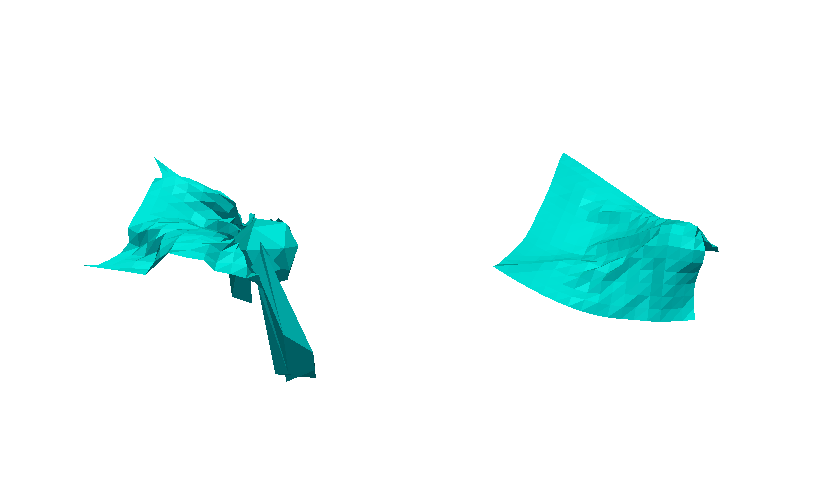
\includegraphics[scale=0.4]{img/comp.png}
 \caption{time step: 0.4s: (L) results before strain limiting step (R) results after strain limiting step}
 \label{fig:1}
\end{figure}

Because of the existence of strain limiting step, even the cloth mesh blows up after physics step,  it can be still refined to a relative reasonable
state by strain limiting as long given a small range of allowed strain bounds whose ends are both close to 1, e.g. [0.9, 1.1].  The refinement of strain limiting is illustrated by figure \ref{fig:1}
under the settings with large time step size.

The strain limiting step does help to improve the stability of the whole simulation, but the refined results may no longer reflect the stability of the dynamical system, 
because the optimization problem \eqref{SL}  is essentially a pure geometric post warping. Therefore, in the next sections, in order to check weather 
our stitch model will bring in the extra instability to the dynamics, we just disable the strain limiting step and only evaluate the numerical stability
of the physics step, i.e. the one-step implicit Euler for the motion equation.

\section{Experiments}
To evaluate the stability of the physics step with and without our stitch model, we use different time steps 
and mesh resolutions as the controlled variables. Figure \ref{fig:nostitch} takes snapshots on the instant that the cloth
without any strips is falling onto a ball. With the time step increasing, the one-time implicit Euler becomes more and more powerless
to generate a smooth deformed configuration and large distortion occurs. Figure \ref{fig:stitch} lists the results corresponding to 
the figure \ref{fig:nostitch} when a single stitch is attached on the cloth, from the last row of which we can see that the solver is still capable of keeping stable even under 
a large time step(0.125) and in a high resolution mesh(64$\times$64), although the results have already distorted a lot. In most simulation, a very large time step
is always impratical because it will result in serious numerical damping, so I think the current model is fairly safe for physically plausible simulation. Figure \ref{fig:final} illustrates the equilibrium state
of the cloth in 64$\times$64 resolutions under the time step of 0.012. As my experiments suggest, multiple strips won't cause big problems either, as showed in figure \ref{fig:multiple}.

\begin{figure}
 \centering
 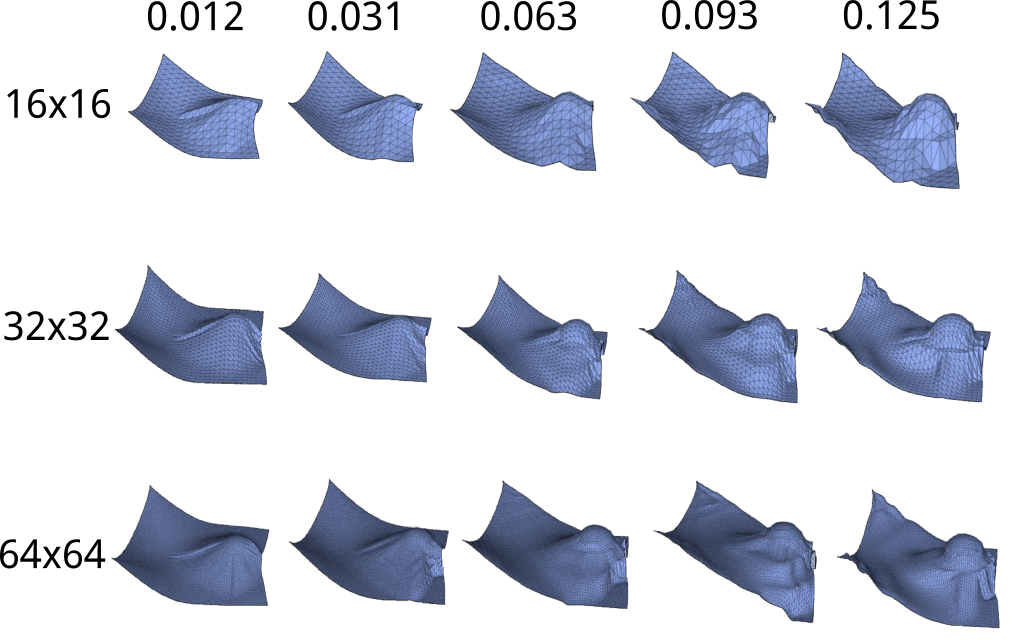
\includegraphics[scale=0.45]{img/without_stitch.png}
 \caption{The mesh in various resolutions simulated under different time step sizes without stitches}
 \label{fig:nostitch}
\end{figure}

\begin{figure}
 \centering
 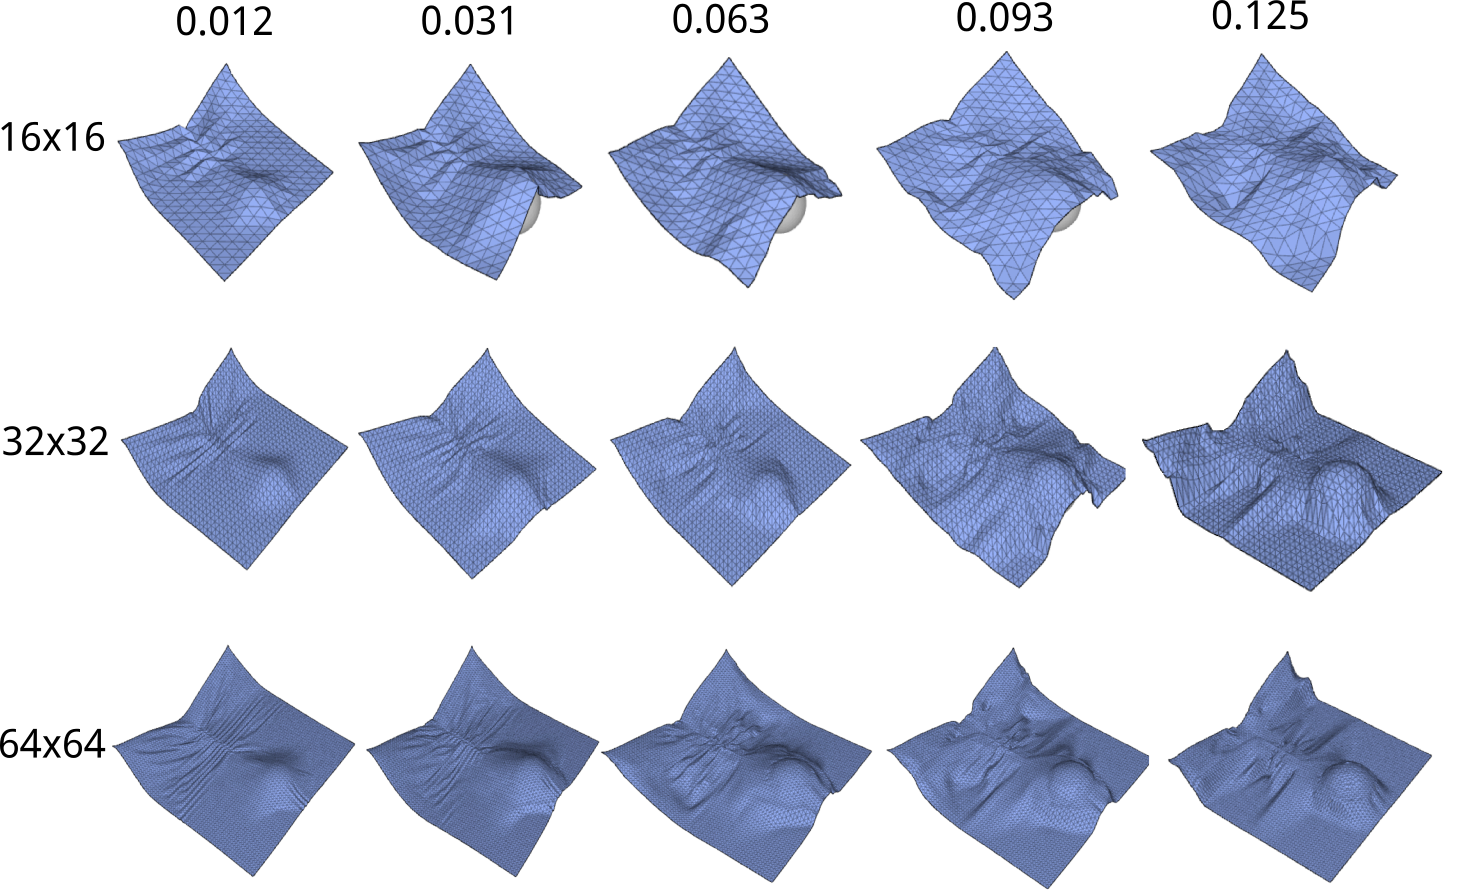
\includegraphics[scale=0.32]{img/with_stitch.png}
 \caption{The mesh with various resolutions simulated under different time step sizes}
 \label{fig:stitch}
\end{figure}

\begin{figure}
 \centering
 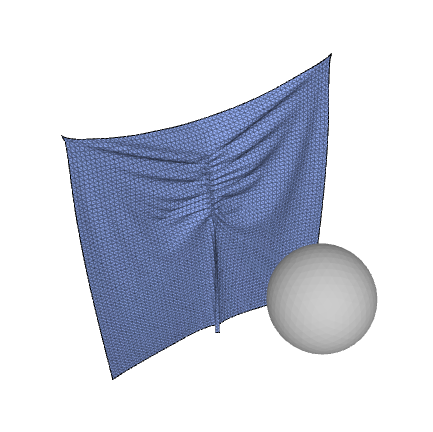
\includegraphics[scale=0.45]{img/final.png}
 \caption{The equilibrium state of 64$\times$64 cloth under gravity}
 \label{fig:final}
\end{figure}

\begin{figure}
 \centering
 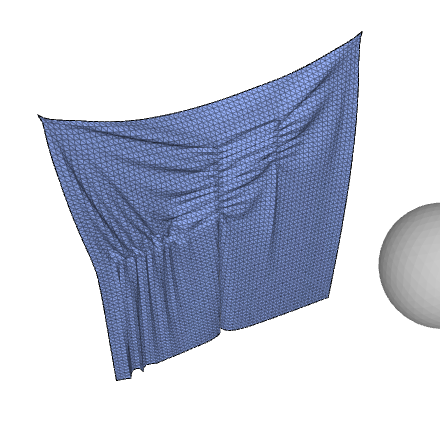
\includegraphics[scale=0.42]{img/multiple_strip.png}
 \caption{The equilibrium state of cloth with three strips}
 \label{fig:multiple}
\end{figure}

\section{Discussions}

I think we need to make the target of the project more clear. 

If what we want is highly realistic simulation, maybe we need to investigate the mechanism behind and derive a convincing constitutive model of the cloth with stitches. 
In this way, the work with the highest priority is to precisely formulate the physical property of the stitch, while choosing a concrete discretization method comes as second.

Suppose our current assumptions on the stitch are reasonable, i.e. almost inextensible and not allowing bending, then the mass spring with large bending penalty is 
sufficient to meet our requirement. According to previous simulation results, this model is not bad to produce the wave pattern along the stitches.
From last section, we can also see that our model won't cause very serious issues on stability, then the question in front of us is if we shall make the simulation more efficient and how.  

The general method to improve the efficiency is to resolve some nonlinearities or reduce the dimensionality. As for the latter one, if we choose to use some generalized coordinates to model the stitches, 
a foreseeable big problem is the coupling of the generalized coordinate system and Euclidean coordinate system, which may involve two-way interactions between stitches and the rest parts of
the cloth and cost even more time to solve. On the other hand, if we manage to remedy this problem and accelerate the simulation of stitches, I'm not sure how much it will improve the overall performance, after all the solve for the dynamics of a large piece of cloth
is always a time consuming job. As we all know, large stiffness will slow the convergence of the iterative solve, but as for physically based simulation, few people is willing to prefer accuracy to speed. 
Since our stitch model only appends some extra terms to internal forces and system matrix, if only iterated once as ARCSim does, there is almost no impact on the efficiency of the physics step.

Suppose that the current simulation is visually satisfying, then another interesting problem is that if there is any approach to seamlessly combine the stitch model and the discontinuous Galerkin element to make the system
more flexible, just as we talked on the first day of starting this project.

According to above discussions, I have some thinkings on our project which could be argued.

\begin{itemize}
 \item To make the simulation more realistic if possible. Maybe we need to consider more geometric and physical properties about the stitch, like width as Prof. Xu suggested or something else.
 \item Efficiency is not the key point here unless the stitches make the solve FAR TOO SLOW.
 \item It is interesting to find a method to make the simulation more flexible, and the stitch model 
 should be adapted to such method in a very natural way.
\end{itemize}

\end{document}
